Negli ultimi decenni, il settore delle costruzioni è stato coinvolto nel processo di evoluzione tecnologica.
Questo ha portato ad un cambio di prospettiva e metodologia operativa, introducendo il Bulding Information Modelling (BIM).
Esso fornisce un insieme di informazioni geometriche, visive, dimensionali, ambientali, tecniche e di processo, rendendo
il processo di progettazione ``sostenibile''.
Il trend è di portare gli applicativi BIM già presenti nel panorama Desktop sul Web, per renderli disponibili anche
sui dispositivi telefonici e portatili. L'obiettivo è cercare di portare dei benifici in termini di disponibilità, affidabilità,
scalabilità, facilità di implementazione, manutenzione e aggiornabilità.

\begin{figure}[htbp] %  figure placement: here, top, bottom, or page
   \centering
   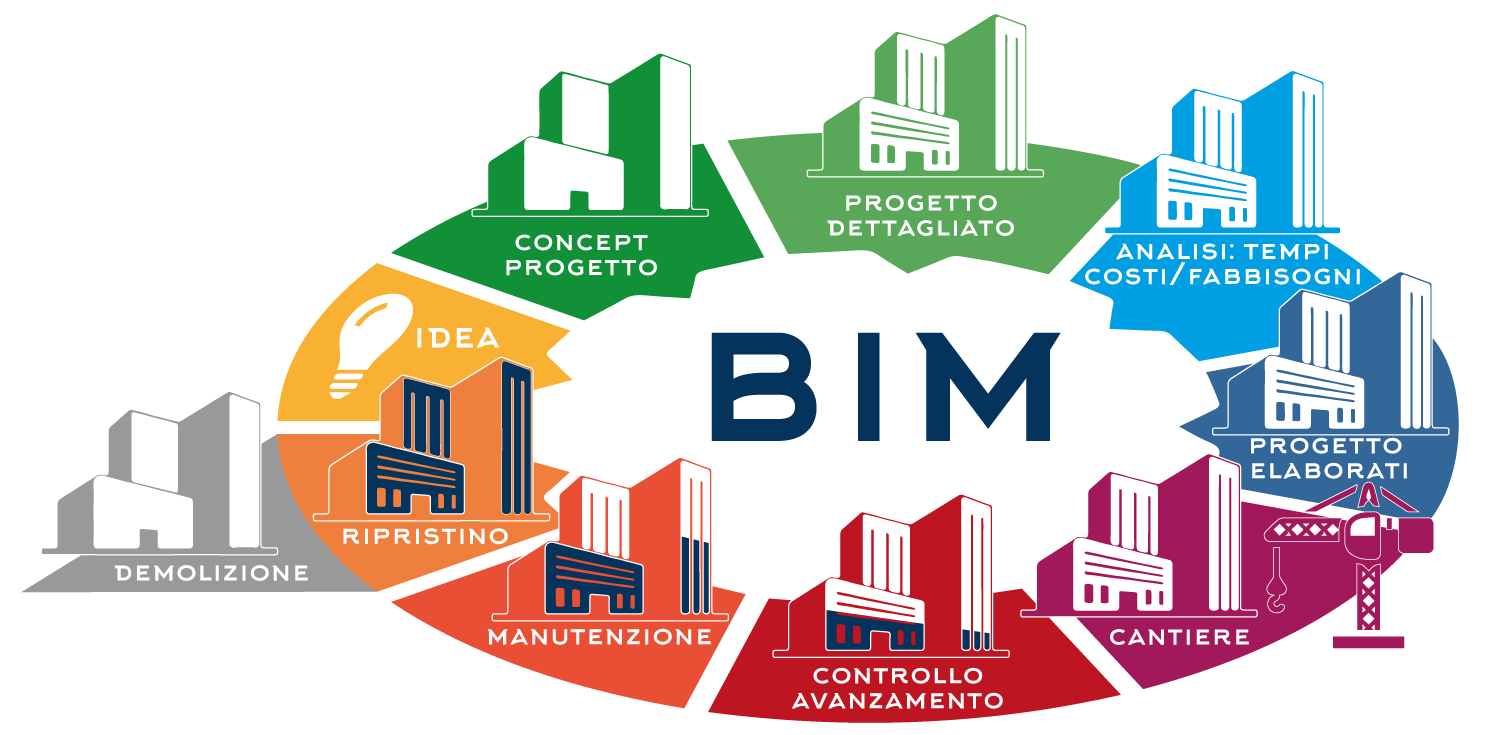
\includegraphics[width=1\linewidth]{images/bim}
   \caption{Fasi coinvolte nel BIM}
   \label{fig:bim}
\end{figure}
\newpage
